\section{Experiment 10H-A: tire-force observer feasibility}
\label{sec:experiment10ha}

\paragraph{Question.}
Experiment 10H assumes access to
$x=[\beta,r,f_{yf},f_{yr},\delta_a]^\top$, where $f_y=F_y/m$. Physical tire
forces and sideslip are not ordinary production measurements. Experiment
10H-A asks whether the latent states can be reconstructed from yaw rate,
lateral acceleration, applied steering, and longitudinal speed, and whether
the estimates are adequate for the frozen 10H LQI controller. This is an
observer feasibility gate, not a federated identification result.

\paragraph{Measurement model and mass interpretation.}
The available output is
\begin{equation}
 y=\begin{bmatrix}r&a_y&\delta_a\end{bmatrix}^\top
 =\begin{bmatrix}
 0&1&0&0&0\\
 0&0&1&1&0\\
 0&0&0&0&1
 \end{bmatrix}x+v.
\end{equation}
Thus $f_{yf}$ and $f_{yr}$ are estimated directly as lateral-acceleration
contributions. Their state definition does not require an externally supplied
mass. Mass remains embedded in the unknown LPV dynamics.

For reference, an algebraic reconstruction follows from
$a_y=f_{yf}+f_{yr}$ and
$(I_z/m)\dot r=l_ff_{yf}-l_rf_{yr}$,
\begin{equation}
 f_{yf}=\frac{l_ra_y+(I_z/m)\dot r}{l_f+l_r},\qquad
 f_{yr}=\frac{l_fa_y-(I_z/m)\dot r}{l_f+l_r}.
\end{equation}
The implemented algebraic baseline is optimistic: it receives the true client
geometry and $I_z/m$ and uses a Savitzky--Golay yaw-acceleration estimate.

\paragraph{Observers and protocol.}
ExactKF uses each client's exact scheduled matrices. GlobalKF uses one matrix
schedule pooled across the fleet and therefore includes plant-model mismatch.
Both measure $r$, $a_y$, and $\delta_a$. The simulated standard deviations are
0.03~deg/s, 0.03~m/s$^2$, and 0.02~deg, with trajectory-constant bias standard
deviations of 0.05~deg/s, 0.04~m/s$^2$, and 0.03~deg. Five process-noise scales
are selected on development seeds 501--505 by a normalized GlobalKF sideslip-
plus-force score. The frozen scale is 0.01. Confirmation uses seeds 511--520.

Every scheduled exact system has observability rank five. The maximum
column-scaled observability condition over all clients and speeds is 196.9,
so the problem is observable and not numerically singular under the assumed
measurements.

\begin{table}[htbp]
\centering
\caption{Experiment 10H-A confirmation estimation accuracy. Force errors are
normalized by the RMS magnitude of the corresponding true contribution.}
\label{tab:experiment10ha-estimation}
\begin{tabular}{lrrr}
\toprule
Method & $\beta$ RMSE [deg] & Front NRMSE & Rear NRMSE\\
\midrule
Algebraic & --     & 6.95\% & 6.47\%\\
GlobalKF  & 0.0483 & 7.96\% & 5.32\%\\
ExactKF   & 0.0091 & 3.72\% & 3.12\%\\
\bottomrule
\end{tabular}
\end{table}

The predefined estimation gates pass: GlobalKF sideslip RMSE is below
0.3~deg, and both axle-force NRMSE values are below 25\%. The class breakdown
identifies the model-mismatch tail. GlobalKF sideslip RMSE is 0.0208~deg for
compact vehicles, 0.0416~deg for sport vehicles, and 0.0825~deg for SUVs;
front-force NRMSE rises to 13.21\% for SUVs.

\paragraph{Output-feedback control test.}
The frozen 10H Global LQI controller is evaluated with FullState, ExactKF, and
GlobalKF feedback. No controller retuning is allowed. The integrator uses
measured yaw rate in the observer cases. Table~\ref{tab:experiment10ha-control}
reports the paired loss of GlobalKF relative to FullState.

\begin{table}[htbp]
\centering
\caption{GlobalKF output-feedback degradation relative to full-state LQI.}
\label{tab:experiment10ha-control}
\begin{tabular}{llrr}
\toprule
Maneuver & Endpoint & Degradation & 95\% CI\\
\midrule
Broadband & Mean client  & 13.08\% & [12.37,13.94]\%\\
Broadband & Worst client & 37.34\% & [34.67,40.38]\%\\
Transient & Mean client  & 20.55\% & [19.75,21.39]\%\\
Transient & Worst client & 44.76\% & [40.16,50.09]\%\\
\bottomrule
\end{tabular}
\end{table}

\begin{figure}[htbp]
\centering
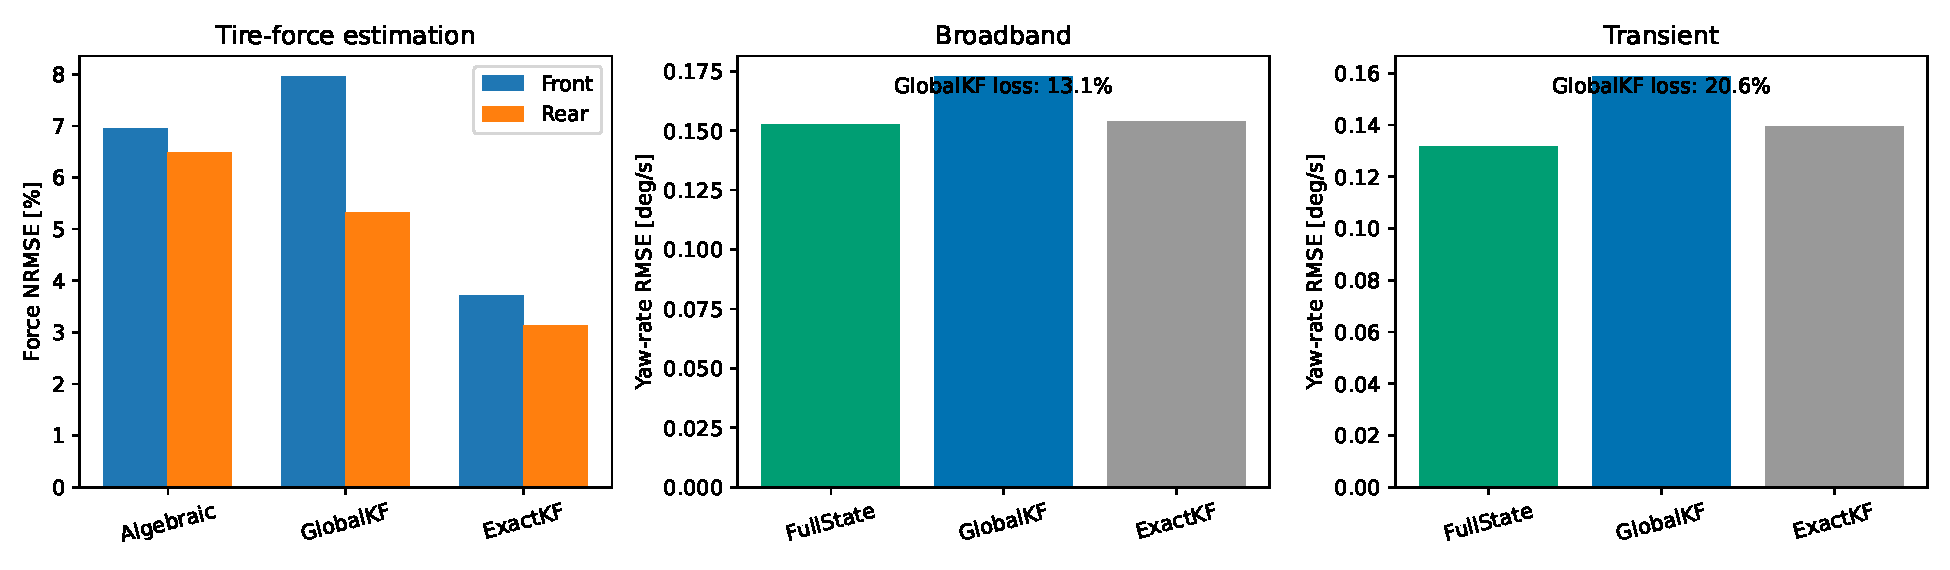
\includegraphics[width=0.98\linewidth]{../results/figures/experiment_10ha_tire_force_observer.pdf}
\caption{Experiment 10H-A estimation accuracy and output-feedback LQI
performance.}
\label{fig:experiment10ha}
\end{figure}

All output-feedback trajectories remain finite, but the control gates fail.
Even ExactKF introduces a smaller control loss, showing that the full-state
LQI gain amplifies estimation noise and bias. GlobalKF adds structured model
mismatch, concentrated in SUV clients, and produces the larger fleet-tail
degradation.

\paragraph{Conclusion and decision.}
Normalized axle-force estimation is feasible from the assumed production-like
signals; unknown absolute mass is not a blocker. However, good state RMSE does
not guarantee acceptable closed-loop performance with the existing aggressive
full-state LQI. We must not use GlobalKF pseudo-states in the next federated
identification experiment without resolving this interface.

The clean next diagnostic is a class-compatible or uncertainty-aware scheduled
observer evaluated with the same frozen LQI, together with an ablation of
sensor bias and observer-model mismatch. If compatible observer sharing closes
the SUV tail without controller retuning, it provides a natural CFL role. If
not, the five-state full-state formulation should be replaced by output-error
LPV identification rather than increasingly complex observer tuning.

\paragraph{Reproducibility.}
Configuration and implementation are in
\path{code/config/experiment_10ha.json} and
\path{code/experiments/experiment_10ha_tire_force_observer.py}. Development
selection, client-level estimation and control records, observability results,
paired intervals, gate decisions, and provenance hashes are stored under
\path{results}.
